\documentclass[10pt]{beamer}

\usepackage{multicol}
\usetheme[progressbar=frametitle]{metropolis}
\usepackage{appendixnumberbeamer}
\usepackage{anyfontsize}
\usepackage{booktabs}
\usepackage[scale=2]{ccicons}
\usepackage{pgfplots}
\usepgfplotslibrary{dateplot}
\usepackage{graphicx}
\usepackage{bussproofs}
\usepackage{xspace}
\usepackage{xcolor}
\newcommand{\themename}{\textbf{\textsc{metropolis}}\xspace}

\usepackage{listings}

\lstset
{ %Formatting for code in appendix
    language=C,
    numbers=left,
    stepnumber=1,
}

%% https://github.com/nickgian/thesis/blob/master/lstcoq.sty
\usepackage{color}

\definecolor{ltblue}{rgb}{0,0.4,0.4}
\definecolor{dkblue}{rgb}{0,0.1,0.6}
\definecolor{dkgreen}{rgb}{0,0.35,0}
\definecolor{dkviolet}{rgb}{0.3,0,0.5}
\definecolor{dkred}{rgb}{0.5,0,0}

% lstlisting coq style (inspired from a file of Assia Mahboubi)
%
\lstdefinelanguage{Coq}{ 
%
% Anything betweeen $ becomes LaTeX math mode
mathescape=true,
%
% Comments may or not include Latex commands
texcl=false, 
%
% Vernacular commands
morekeywords=[1]{Section, Module, End, Require, Import, Export,
  Variable, Variables, Parameter, Parameters, Axiom, Hypothesis,
  Hypotheses, Notation, Local, Tactic, Reserved, Scope, Open, Close,
  Bind, Delimit, Definition, Let, Ltac, Fixpoint, CoFixpoint, Add,
  Morphism, Relation, Implicit, Arguments, Unset, Contextual,
  Strict, Prenex, Implicits, Inductive, CoInductive, Record,
  Structure, Canonical, Coercion, Context, Class, Global, Instance,
  Program, Infix, Theorem, Lemma, Corollary, Proposition, Fact,
  Remark, Example, Proof, Goal, Save, Qed, Defined, Hint, Resolve,
  Rewrite, View, Search, Show, Print, Printing, All, Eval, Check,
  Projections, inside, outside, Def},
%
% Gallina
morekeywords=[2]{forall, exists, exists2, fun, fix, cofix, struct,
  match, with, end, as, in, return, let, if, is, then, else, for, of,
  nosimpl, when},
%
% Sorts
morekeywords=[3]{Type, Prop, Set, true, false, option},
%
% Various tactics, some are std Coq subsumed by ssr, for the manual purpose
morekeywords=[4]{pose, set, move, case, elim, apply, clear, hnf,
  intro, intros, generalize, rename, pattern, after, destruct,
  induction, using, refine, inversion, injection, rewrite, setoid_rewrite, congr,
  unlock, compute, ring, field, fourier, replace, setoid_replace, fold, unfold,
  change, cutrewrite, simpl, have, suff, wlog, suffices, without,
  loss, nat_norm, assert, cut, trivial, revert, bool_congr, nat_congr,
  symmetry, transitivity, auto, split, left, right, autorewrite},
%
% Terminators
morekeywords=[5]{by, done, exact, reflexivity, tauto, romega, omega,
  assumption, solve, contradiction, discriminate},
%
% Control
morekeywords=[6]{do, last, first, try, idtac, repeat},
%
% Comments delimiters, we do turn this off for the manual
morecomment=[s]{(*}{*)},
%
% Spaces are not displayed as a special character
showstringspaces=false,
%
% String delimiters
morestring=[b]",
morestring=[d]’,
%
% Size of tabulations
tabsize=3,
%
% Enables ASCII chars 128 to 255
extendedchars=false,
%
% Case sensitivity
sensitive=true,
%
% Automatic breaking of long lines
breaklines=false,
%
% Default style fors listings
basicstyle=\small,
%
% Position of captions is bottom
captionpos=b,
%
% flexible columns
basewidth={2em, 0.5em},
columns=flexible,
%
% Style for (listings') identifiers
identifierstyle={\ttfamily\color{black}},
% Style for declaration keywords
keywordstyle=[1]{\ttfamily\bfseries\color{dkviolet}},
% Style for gallina keywords
keywordstyle=[2]{\ttfamily\bfseries\color{dkgreen}},
% Style for sorts keywords
keywordstyle=[3]{\ttfamily\bfseries\color{ltblue}},
% Style for tactics keywords
keywordstyle=[4]{\ttfamily\color{dkblue}},
% Style for terminators keywords
keywordstyle=[5]{\ttfamily\color{dkred}},
%Style for iterators
%keywordstyle=[6]{\ttfamily\color{dkpink}},
% Style for strings
stringstyle=\ttfamily,
% Style for comments
commentstyle={\ttfamily\itshape\color{dkgreen}},
%
%moredelim=**[is][\ttfamily\color{red}]{/&}{&/},
literate=
    {fun}{{\color{dkgreen}{$\lambda\;$}}}1
    {bool}{{$\mathbb{B}$}}1
    {nat}{{$\mathbb{N}$}}1
    {Vforall2}{Vforall2}1 % quick workardoun to avoid partial replacement of 'forall' in identifier
    {nat\_equiv}{nat\_equiv}1 % quick workardoun to avoid partial replacement of 'nat' in identifier
    {forall}{{\color{dkgreen}{$\forall\;$}}}1
    {exists}{{$\exists\;$}}1
    {<-}{{$\leftarrow\;\;$}}1
    {=>}{{$\Rightarrow\;\;$}}1
    {==}{{\texttt{==}\;}}1
    {==>}{{$\Longrightarrow\;\;$}}1
%    {:>}{{\texttt{:>}\;}}1
    {->}{{$\rightarrow\;\;$}}1
    {<-->}{{$\longleftrightarrow\;\;$}}1
    {<->}{{$\leftrightarrow\;\;$}}1
    {<==}{{$\leq\;\;$}}1
    {\#}{{$^\star$}}1 
    {\\o}{{$\circ\;$}}1 
%    {\@}{{$\cdot$}}1 
    {\/\\}{{$\wedge\;$}}1
    {\\\/}{{$\vee\;$}}1
    {++}{{\texttt{++}}}1
    {~}{{\ }}1
    {¬}{{$\lnot$}}1     % this does not work
    {\@\@}{{$@$}}1
    {\\mapsto}{{$\mapsto\;$}}1
    {\\hline}{{\rule{\linewidth}{0.5pt}}}1
%
}[keywords,comments,strings]

\lstnewenvironment{coq}{\lstset{language=Coq}}{}

% pour inliner dans le texte
\def\coqe{\lstinline[language=Coq, basicstyle=\small]}
% pour inliner dans les tableaux / displaymath...
\def\coqes{\lstinline[language=Coq, basicstyle=\scriptsize]}

%%% Local Variables: 
%%% mode: latex
%%% Local IspellDict: british
%%% TeX-master: "main.tex"
%%% End: 

\title{Formal Verification of Computer Programs}
\subtitle{A Primer}
% \date{\today}
\date{\date{}}
\author[shortname]{Vadim Zaliva \textsuperscript{1} \and Nika Pona \inst{2}}
\institute[shortinst]{\textsuperscript{1}Carnegie Mellon  University \and \inst{2} Digamma.ai}

% \titlegraphic{\hfill\includegraphics[height=1.5cm]{logo.pdf}}

\begin{document}

\maketitle

\begin{frame}{Table of contents}
  \setbeamertemplate{section in toc}[sections numbered]
  \tableofcontents[hideallsubsections]
\end{frame}


\section{What are formal methods?}
\begin{frame}{Formal verification}
 
  We want to have high assurance that the code we wrote works as intended and is bug-free. One of the methods to do this is {\bf formal verification}, which amounts to producing {\it a formal proof} of correctness.

  {\center What does it mean and how do we do it?}
  
  \begin{enumerate}
  \item We write the \emph{specification} in {\it a formal language} which unambiguously defines how our program should behave.
  \item Then we model our program and its actual behaviour, that is, we define the \emph{semantics} of our program. 
  \item Finally we mathematically prove that the behaviour of our program matches the specification.
\end{enumerate}

In what follows we will talk about formal verfication using {\bf Coq proof assistant}.
  
\end{frame}

\section{Verifying C code: a motivating example}

\begin{frame}{\texttt{asn\_strtoimax\_lim} of ASN.1C compiler}
  At \url{Digamma.ai} we are working on formal verification of existing {\bf imperative} programs using Coq. We took a function \texttt{asn\_strtoimax\_lim} from \texttt{asn1c} compiler to test our approach on a simple real-life example.
  

  Informal specification from the comments: 

 \begin{quote}
 Parse the number in the given string until the given *end position,
 returning the position after the last parsed character back using the
 same (*end) pointer.
 WARNING: This behavior is different from the standard strtol/strtoimax(3).
\end{quote}
\end{frame}

\begin{frame}{\texttt{asn\_strtoimax\_lim} code}
  
  {\fontsize{4}{1}\selectfont  \lstinputlisting[language=C]{asn_strtoimax_lim_old.c}}
  
\end{frame}


\begin{frame}{\texttt{asn\_strtoimax\_lim}}

   During correctness proof, some proof obligations about the for loop were produced that could not be met, because of a bug in the function. Can you see it?

  \url{https://github.com/vlm/asn1c/issues/344}
  
\end{frame}

\begin{frame}{Negative error range bug}

When we go beyond allowed int range, a false result is given on some inputs:  

input: -9223372036854775809 \\
intmax: 9223372036854775807 \\
upper boundary: 922337203685477580 \\
last digit max: 7\\
ASN\_STRTOX\_ERROR\_RANGE\\

\bigskip

input: -9223372036854775810 \\
intmax: 9223372036854775807 \\
upper boundary: 922337203685477580 \\ 
last digit max: 7 \\
output: 70 \\
ASN\_STRTOX\_OK


\end{frame}

\begin{frame}{Negative error range bug}
    This happens whenever the input string represents a number smaller than \texttt{MIN\_INT}, due to the fact that absolute value of \texttt{MIN\_INT} is greater than \texttt{MAX\_INT}, thus negative number cannot be treated as value * sign. 
    
    Formal proof has to cover all cases, hence this bug became obvious during the proof.
    
\end{frame}{}

\begin{frame}{\texttt{asn\_strtoimax\_lim} fixed}
  
    {\fontsize{4}{1}\selectfont \lstinputlisting[language=C]{asn_strtoimax_lim.c}}

\end{frame}
  
  \begin{frame}[fragile]{\texttt{asn\_strtoimax\_lim} fixed}

    Is this fix OK? Look at this part of the code: 

     \begin{lstlisting}[language=C]
  if(str < *end) {
    *end = str;
    if(*str >= 0x30 && *str <= 0x39){
      return ASN_STRTOX_ERROR_RANGE;
    } else {
      *intp = sign * value;
      return ASN_STRTOX_EXTRA_DATA;
    }
  }
  \end{lstlisting}
  
\end{frame}

\begin{frame}{Memory store bug}

    Let minimal signed int \texttt{MIN\_INT} = $-4775808$ 

    \texttt{*str} = {\color{red}2d 34 37 37 35 38 30 31 31 31} ( stands for ``-477580111'') 

    \paragraph{{\bf Scenario 1}:}

    Assume that \texttt{*end = *(str + 9)} and  \texttt{end} points outside of \texttt{*str}.

     {\color{red}2d 34 37 37 35 38 30 {\color{blue}$\overbrace{31}^{\texttt{*(str + 7)}}$} 31 31 $\ldots$ $\overbrace{\texttt{X}}^{\texttt{*end}}$}

     Then at \texttt{*(str + 7)} we store \texttt{*end = (str + 7)}

     Let \texttt{(str + 7) = 21 21 21 26} 

     {\color{red}2d 34 37 37 35 38 30 31 {\color{blue} $\overbrace{31}^{\texttt{*(str + 8)}}$} 31  $\ldots$ $\overbrace{\texttt{21 21 21 26}}^{\texttt{*end}}$}
     
     And since at \texttt{*(str + 8)} we read ``1''
     

     
     The output is  \texttt{ASN\_ERROR\_RANGE}.


  \end{frame}

  \begin{frame}{Memory store bug}

    Let minimal signed int \texttt{MIN\_INT} = $-4775808$ 

    \texttt{*str} = {\color{red}2d 34 37 37 35 38 30 31 31 31} (stands for ``-477580111'') 

    \paragraph{{\bf Scenario 2}:}

    Assume that \texttt{*end = *(str + 9)} and \texttt{end} points inside of \texttt{*str}:
    
    {\color{red}2d 34 37 37 35 38 {\color{blue} $\overbrace{30 \; 31 \; 31 \; 31}^{\texttt{*end}}$}}
    

    Then at \texttt{*(str + 7)} we store \texttt{*end = (str + 7)}

     Let \texttt{(str + 7) = 21 21 21 26} 

   
    {\color{red}2d 34 37 37 35 38 30 {\color{blue}$\overbrace{21 \; 21 \; 21 \; 26}^{\texttt{*end}}$}}
    (stands for $``-477580!!!\&''$)

    And since at \texttt{*(str + 8)} we read ``!'' 

    The output is \texttt{ASN\_EXTRA\_DATA}.
    
    \end{frame}



\begin{frame}{\texttt{asn\_strtoimax\_lim}}
   This configuration may happen only on some hardware architectures and almost impossible to reproduce. Yet, the vulnerability is there and posses a potential problem.
   
  This code has been extensively tested and used for 15 years. Formal verification guarantees absence of these kind of bugs.

  

\end{frame}

\section{Coq mini-intro}

\begin{frame}{Coq mini-intro}
  We did our proofs in a formal language we choose {\it Gallina}, a mechanized version of {\bf Calculus of Inductive Constructions}, which is a very expressive type theory well studied in mathematical logic. We write the specifications, model our programs and do the proofs in this language.

  \smallskip
We could do all of the above on paper, but it would quickly get out of hand. Moreover, we want to be sure that there are no mistakes in the proofs.
  
  So we use a tool called {\bf proof assistant}: a program that checks that your proof is correct. It also provides an environment to make the construction of proofs easier. In particular, we will talk about the Coq proof assistant: \url{https://coq.inria.fr/}.
  
  
\end{frame}

\begin{frame}{What Coq does?}
  In Coq you can:
  \begin{itemize}
  
    \item define functions and predicates
   \item state mathematical theorems and software specifications
    \item interactively develop formal proofs of theorems
   \item machine-check these proofs by a relatively small certification kernel
    \item extract certified programs to languages like OCaml, Haskell or Scheme.
  \end{itemize}
  

\end{frame}


\begin{frame}[fragile]{Inductive definitions}

  In Coq everything is either a {\it term} or a {\it type}. You can define basic inductive types using the \texttt{Inductive} command.

  \begin{lstlisting}[language=Coq]
  Inductive bool : Set :=
    | true : bool
    | false : bool.

  \end{lstlisting}

  The boolean type has two {\bf constructors}: \texttt{true} and \texttt{false}.  
  
   \begin{lstlisting}[language=Coq]
  Inductive nat : Set :=
    | O : nat
    | S : nat -> nat.  
   \end{lstlisting}

   Natural numbers are defined by two constructors as well: \texttt{O} (zero) and \texttt{S} (successor function). Any {\it term} of type $\mathbb{N}$ is constructed using these two. E.g., \texttt{S O} : $\mathbb{N}$, \texttt{S (S O)} : $\mathbb{N}$, \texttt{S (S (S O))} : $\mathbb{N}$  \ldots
\end{frame}

\begin{frame}[fragile]{Recursive definitions}

  You can define recursive functions using the \texttt{Fixpoint} command.

  Since we know that by construction any term of type $\mathbb{N}$ is either \texttt{O} or \texttt{S n} for some $n : \mathbb{N}$, we can use {\it pattern-matching}.
  
   \begin{lstlisting}[language=Coq]
  Fixpoint plus (n m : nat) : nat :=
  match n with
  | O => m
  | S p => S (plus p m)
  end
   \end{lstlisting}
   
Note: Coq only accepts definitions that terminate\footnote{This limitation is needed to ensure consistency of the system, as well as decidability of type-checking.}. Here we are recursing on a direct subterm of $n$ thus we are guaranteed to terminate and Coq is able to automatically ensure this. Sometimes you have to do a termination proof by hand. 
\end{frame}


\begin{frame}[fragile]{Proofs}


  Finally, you can state and prove theorems about the objects you defined. Let $+$ be notation for \texttt{plus}.

  \begin{theorem} 2 + 3 = 5.
    \end{theorem}

  How would you prove this, if you were to justify each step of the proof?
  
  \begin{lstlisting}[language=Coq]
Theorem plus_2_3 : (S (S O)) + (S (S (S O))) = (S (S (S (S (S O))))).
 Proof.
  unfold plus. (* apply definition of plus *)
  reflexivity. (* apply definition of equality *)
 Qed.

  \end{lstlisting}
  In Coq you constructs a proof using so-called {\sf tactics}.
  E.g., \texttt{simpl} is a tactic that performs basic application of definitions, \texttt{reflexivity} proves equality between two syntactically equal terms (modulo some reductions).  
 
\end{frame}


\begin{frame}[fragile]{More proofs}
\begin{theorem} $\forall n \; (0 + n = n)$.
\end{theorem}

To prove this we also use the definition of addition: since the recursion is on the first term, we are in the base case.

   \begin{lstlisting}[language=Coq]
  Fixpoint plus (n m : nat) : nat :=
  match n with
  | O => m (* base case *)
  | S p => S (plus p m)
  end
   \end{lstlisting}

   Proof in Coq:

  \begin{lstlisting}[language=Coq]
    Theorem plus_O_n : (forall n, O + n = n).
    Proof.
      intros n. (* take any n *)
      simpl. (* apply definition of plus *)
      reflexivity. (* get equal terms *)
    Qed.
  \end{lstlisting}

 
\end{frame}



\begin{frame}[fragile]{More proofs}

  Most proofs would need to go by induction (Why the previous proof won't work below? See how \texttt{plus} is defined.)

  \begin{lstlisting}[language=Coq]
    Theorem plus_n_O : (forall n, n + O = n).
    Proof.
      (* proof by induction on n *)
      induction n; simpl.
      (* base case *)
      - reflexivity.
      (* inductive step *)
      - rewrite IHn. (* apply induction hypothesis *)
        reflexivity.
    Qed.

  \end{lstlisting}
\end{frame}
\begin{frame}{More Proofs}
     In Coq you have to justify every step of the proof and the \texttt{Qed} command only succeeds on correct proofs. But you don't have to do every proof from scratch, since there are extensive libraries covering lemmas about basic mathematics as well as several decision procedures that automatize proof search.
     \begin{itemize}
     \item Using SMT and SAT solvers: \url{https://smtcoq.github.io/}
     \item First-order decision procedures (CoqHammer): \url{https://github.com/lukaszcz/coqhammer}
     \item Tactics for solving arithmetic goals over ordered rings (\texttt{Micromega})
       \item And much more, cf. \url{https://coq.inria.fr/opam/www/}
       \end{itemize}
  
\end{frame}

   \section{How does Coq work?}
\begin{frame}{How does Coq work?}
    We can formalize programs, properties and proofs in the same language, as well as efficiently and reliably check proof correcteness due to the so-called {\bf Curry-Howard isomorphism}.

    Curry-Howard isomorphism is a correspondence between programs and terms on one hand and proofs and types on the other. All logical statements in Coq are typing judgments and thus checking the correctness of proofs amounts to type checking. Let's see what it means precisely on a small example.
   \end{frame}
   
   \begin{frame}{Curry-Howard Isomorphism (CHI)}
     We said that {\it ``Curry-Howard isomorphism is a correspondence between programs and terms on one hand and proofs and types on the other''}. To make this precise, we need to specify what kind of programs we have on one side and what kind of proofs (that is, what kind of logic) we have on the other side.

     Various {\bf lambda calculi} were designed to describe programs.% {\it untyped lambda-calculus, simply-typed lambda calculus, polymorphic lambda-calculus, G\"{o}del's system {\bf T}, system {\bf F}} etc\footnote{cf. Lectures on Curry-Howard Isomorphism \cite{Sørensen98lectureson}}.
     If you never heard of lambda calculi, think of functional programming languages such as {\bf OCaml} and {\bf Haskell}.
     
\end{frame}
\begin{frame}{The simplest CHI: simply typed lambda calculus}
    Consider the simplest example of typed lambda calculus\footnote{Or a rudimentary functional programming language.}: simply typed lambda calculus {\bf ST}. Terms of {\bf ST} are:
     \begin{description}
     \item[Var] variables
     \item[Abs] $(\lambda x.M)$, if $x$ a variable and $M$ is a term 
     \item[App] $(M N)$, if $M$ and $N$ are terms
     \end{description}
     Think of $(\lambda x.M)$ as a function with argument $x$ and body $M$ and of $(M N)$ as applying function $M$ to the argument $N$. %This is formalized by introducing $\beta$-{\it reduction} relation on terms:
     %\[ (\lambda x.M)N \Rightarrow_\beta M[x := N]\footnote{Meaning substitute all occurences of x in M by N.} \] 
%Some examples of $\beta$-reduction: 
 %    \[ (\lambda x.x)y \Rightarrow_\beta y \]
  %   \[ ((\lambda x.(x z)) y \Rightarrow_\beta (y z) \]

\end{frame}
\begin{frame}{Simply typed lambda calculus}
       
     In lambda calculus one could encode basic data types such as natural numbers and lists, as well as functions on them and logical constants and operations. {\bf ST} could be extended with a fixpoint operator to allow for recursive functions.

     Examples of terms:

     $\lambda x.x$ (identity function)
     
     $\lambda x.\lambda y. x$ (true\footnote{By convention: you could define constants in a different way as well.})

     $\lambda x.\lambda y. y$ (false or zero)

     $\lambda n. \lambda y. \lambda x. y (n y x)$ (successor function)
\end{frame}
\begin{frame}{Simply typed lambda-calculus}
       We are interested in a {\bf typed} lambda calculus. The types of {\bf ST} are:
        \begin{description}
     \item[Var] type variables 
     \item[Arrow] $\tau \rightarrow \sigma$, if $\tau$ and $\sigma$ are types
       \end{description}
       Types are assigned to terms according to certain rules. Let $\Gamma$ be a set of simply-typed terms (also called context). 
       \begin{prooftree}
          \AxiomC{$\Gamma, x : \tau \vdash x : \tau $ ({\bf Ax})}     
                 \end{prooftree}

         \begin{prooftree}
           \AxiomC{$\Gamma, x : \sigma \vdash M : \tau$}
           \RightLabel{({\bf Abs})}
           \UnaryInfC{$\Gamma \vdash (\lambda x. M) : \sigma \rightarrow \tau$}
         \end{prooftree}

         \begin{prooftree}
           \AxiomC{$\Gamma \vdash M : \sigma \rightarrow \tau$}
           \AxiomC{$\Gamma \vdash N : \sigma$}
           \RightLabel{({\bf App})}
           \BinaryInfC{$\Gamma \vdash (M N) : \tau$}
         \end{prooftree}
\end{frame}
\begin{frame}{Simply typed lambda-calculus}
         Here is a simple derivation that shows that the term $\lambda x. x$ (identity) has type $\sigma \rightarrow \sigma$, with $\sigma$ being any type of {\bf ST}: \begin{prooftree}
          \AxiomC{$ x : \sigma \vdash x : \sigma$ ({\bf Ax})}
          \RightLabel{({\bf Abs})}
           \UnaryInfC{$\vdash (\lambda x. x) : \sigma \rightarrow \sigma$}
         \end{prooftree}

And if you apply identity to a term of type $\sigma$, the output is also of type $\sigma$:

\begin{prooftree}
          \AxiomC{$ y : \sigma, x : \sigma \vdash x : \sigma$ ({\bf Ax})}
          \RightLabel{({\bf Abs})}
           \UnaryInfC{$y : \sigma, \vdash (\lambda x. x) : \sigma \rightarrow \sigma$}
           \AxiomC{ $y : \sigma \vdash y : \sigma$ ({\bf Ax})}
           \RightLabel{({\bf App})}
           \BinaryInfC{ $y : \sigma \vdash ((\lambda x. x) y) : \sigma$}
         \end{prooftree}
         \end{frame}
         
\begin{frame}<0>
A more complex example.         
          \begin{prooftree}
            \AxiomC{$y : \tau, x : \tau \rightarrow \sigma \vdash x : \tau \rightarrow\sigma$ ({\bf Ax})}
            \AxiomC{$y : \tau, x : \tau \rightarrow \sigma \vdash y : \tau$ ({\bf Ax}) }
          \RightLabel{({\bf App})}
          \BinaryInfC{$y : \tau, x : \tau \rightarrow \sigma  \vdash (x y) : \sigma$}
          \RightLabel{({\bf Abs})}
          \UnaryInfC{$ y : \tau \vdash \lambda x. (x y) : (\tau \rightarrow \sigma) \rightarrow \sigma$}
          \RightLabel{({\bf Abs})}
          \UnaryInfC{$\vdash \lambda y.\lambda x. (x y) : \tau \rightarrow (\tau \rightarrow \sigma) \rightarrow \sigma$}
         \end{prooftree}
\end{frame}
\begin{frame}{Back to CHI}
         We made one side of the Curry-Howard correspondence more precise: the simply typed lambda calculus, which corresponds to some rudimenatry functional programming language. Now: what does it correspond to and how?

         In general programs (or computations) will correspond to certain kind of logics. Namely, {\bf intuitionistic logics}. These logics were created to formalize what is called constructive mathematics: that is, mathematics in which we are only interested in objects that can be effectively constructed.
\end{frame}
   
\begin{frame}{Implicational propositional logic}
     Consider the simplest intuitionistic logic {\bf Impl}. The formulae of {\bf Impl} are the following: 
     \begin{description}
     \item[Var] propositional variables 
     \item[Impl] $\tau \rightarrow \sigma$, for $\tau, \sigma$ propositional formulae
       \end{description}

     Examples of formulae: $p \rightarrow p$, $p \rightarrow (q \rightarrow p)$.

     Let $\Gamma$ be a set of formulae.  The theorems of {\bf Impl} are proved according to the following rules of inference:
       \[ \Gamma, \phi \vdash \phi \; ({\bf Ax}) \]

         \begin{prooftree}
           \AxiomC{$\Gamma, \phi \vdash \psi$}
                      \RightLabel{($\rightarrow$-I)}
           \UnaryInfC{$\Gamma \vdash \phi \rightarrow \psi$}
         \end{prooftree}

         \begin{prooftree}
           \AxiomC{$\Gamma \vdash \phi \rightarrow \psi$}
           \AxiomC{$\Gamma \vdash \phi$}
            \RightLabel{($\rightarrow$-E)}
           \BinaryInfC{$\Gamma \vdash \psi$}
         \end{prooftree}
\end{frame}

  

\begin{frame}{Curry-Howard Isomorphism}
       You may notice a parallelism between the rules of inference of {\bf Impl} and typing rules of simply typed lambda-calculus, this is the core of Curry-Howard Isomorphism.

\begin{multicols}{2}

          \begin{prooftree}
          \AxiomC{$\Gamma,  \phi \vdash \phi $ ({\bf Ax})}     
                 \end{prooftree}
                 
                  \begin{prooftree}
          \AxiomC{$\Gamma, x : \tau \vdash x : \tau $ ({\bf Ax})}     
         \end{prooftree}

                 \end{multicols}

         
\begin{multicols}{2}
\begin{prooftree}
           \AxiomC{$\Gamma, \phi \vdash \psi$}
                      \RightLabel{($\rightarrow$-I)}
           \UnaryInfC{$\Gamma \vdash \phi \rightarrow \psi$}
         \end{prooftree}


         

         \begin{prooftree}
           \AxiomC{$\Gamma, x : \sigma \vdash M : \tau$}
           \RightLabel{({\bf Abs})}
           \UnaryInfC{$\Gamma \vdash (\lambda x. M) : \sigma \rightarrow \tau$}
         \end{prooftree}

        
\end{multicols}

\begin{multicols}{2}

\begin{prooftree}

           \AxiomC{$\Gamma \vdash \phi \rightarrow \psi$}
           \AxiomC{$\Gamma \vdash \phi$}
            \RightLabel{($\rightarrow$-E)}
           \BinaryInfC{$\Gamma \vdash \psi$}
         \end{prooftree}
 \begin{prooftree}
           \AxiomC{$\Gamma \vdash M : \sigma \rightarrow \tau$}
           \AxiomC{$\Gamma \vdash N : \sigma$}
           \RightLabel{({\bf App})}
           \BinaryInfC{$\Gamma \vdash (M N) : \tau$}
         \end{prooftree}
         
         \end{multicols}

\end{frame}
\begin{frame}{Curry-Howard Isomorphism}

  Consider {\bf ST} with type variables being propositional variables; then types are formulae of {\bf Impl}. We can show that:
\begin{theorem}[CHI]
  A simple lambda term $M$ has a type $\tau$ in {\bf ST} if and only if $\tau$ is provable in {\bf Impl}.
  \end{theorem}
\end{frame}


      

      

    

\begin{frame}{Curry-Howard Isomorphism}
             You've seen the simplest type theory and propositional logic and how Curry-Howard Isomorphism works.
    
             Now we can expand {\bf ST} to include more terms and types (you can allow sum and product types, polymorphism, recursors - which allows you to formulate more functions) or alternatively expand the logic to be more expressible and complex (add other
             connectives, quantifiers, inductive definitions etc).
    
             But the principle stays the same and you have Curry-Howard Isomorphism for very complex type systems, such as Calculus of Inductive Constructions, on which Coq is based. 
\end{frame}

\begin{frame}{Curry-Howard Isomorphism}
       
       \begin{tabular}{ l | r }
         {\bf logic } & {\bf lambda-calculus} \\
         \hline
         formula & type  \\
         proof & term \\
         propositional variable & type variable  \\
         implication & function space  \\
         conjunction & product \\
         disjunction & disjoint sum \\
         absurdity & empty type \\
         normalization & reduction \\
         provability & type inhabitation \\      
       \end{tabular}
\end{frame}
       
\begin{frame}<0>[fragile]{Proofs as functional programs}

  Let's return to one of our first proofs:

  \begin{lstlisting}[language=Coq]
    Theorem plus_O_n : (forall n, O + n = n).
    Proof.
      intros n.
      simpl.
      reflexivity.
    Qed.

  \end{lstlisting}

  By Curry-Howard Isomorphism, the proof of this statement corresponds to constructing a term, that is, to writing a functional program.

   \begin{lstlisting}[language=Coq]
    plus_O_n = fun n : nat => eq_refl
     : forall n : nat, O + n = n
  \end{lstlisting}

 with \texttt{eq\_refl} being a term of type \texttt{x = x}.
  
\end{frame}

\begin{frame}[fragile]{Proofs as functional programs}
  \begin{lstlisting}[language=Coq]
    Theorem plus_n_O : (forall n, n + O = n).
    Proof.
      induction n; simpl.
      - reflexivity.
      - rewrite IHn. 
      reflexivity.
    Qed.
  \end{lstlisting}
By Curry-Howard Isomorphism, the proof of this statement corresponds to constructing a term, that is, to writing a functional program.
  \begin{lstlisting}[language=Coq]
    plus_n_O = fun n : nat =>
               nat_ind (fun n0 : nat => n0 + O = n0) eq_refl
               (fun (n0 : nat) (IHn : n0 + O = n0) =>
                eq_ind_r (fun n1 : nat => S n1 = S n0) eq_refl IHn) n
    : forall n : nat, n + O = n
  \end{lstlisting}
  where \texttt{nat\_ind} is a term with type that corresponds to induction on natural numbers and \texttt{eq\_refl} being a term of type \texttt{x = x}.

\end{frame}
\begin{frame}{Coq's kernel}
  Since the logic we are dealing with is more complex than {\bf Impl}, the functional programs corresponding to these types are also way more complex. However, checking whether a given term $t$ has a given type $\sigma$ is a decidable problem even for Calculus of Inductive Constructions. By Curry-Howard Isomorphism, this also yields a procedure for checking the correctness of proofs written in Coq's logic.  This algorithm constitutes Coq's trusted {\bf kernel}.

\end{frame}

\begin{frame}{Coq's architecture}
    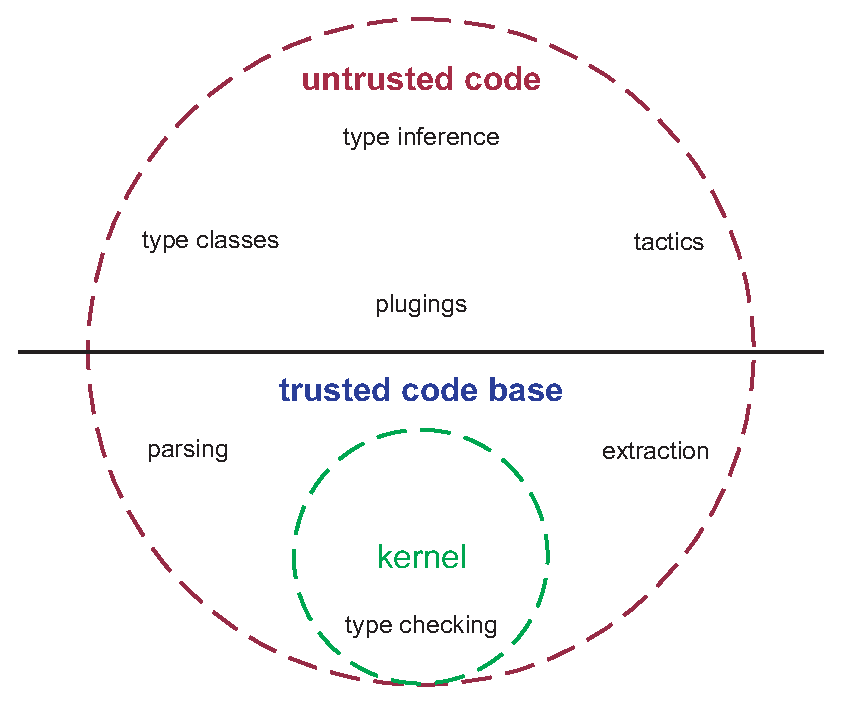
\includegraphics[width=9cm,height=7cm]{pictures/circ.eps}
    \cite{SozeauPic}
\end{frame}

\begin{frame}
 Now we will see how Coq is used for verifying programs.
\end{frame}



\section{Verifying C code: a detailed example}


\begin{frame}[fragile]{Factorial example}
  Mathematical specification of factorial is a recursive equation, for ($0 \leq n$):
  \begin{align*}
  fact(0) &= 1 \\
  fact(n + 1) &= fact(n)*(n+1)    
  \end{align*}
  We can write it in Coq as a fixpoint definition:
  \begin{lstlisting}[language=Coq]
  Fixpoint fact (n : nat) : nat :=
    match n with
    | O => 1
    | S n' => n * fact n'
    end.
  \end{lstlisting}
  Note that this definition is also a functional program\footnote{This corresponds to the idea of verifying a program wrt reference implementation. For more complex program we will want to write a specification in a more declarative fashion.}.
 
\end{frame}



\begin{frame}[fragile]{Factorial example: verifying a functional program}

  We can write a more efficient (tail-recursive) functional program to compute factorial

  \begin{lstlisting}[language=Coq]
  Fixpoint fact_acc (n : nat) (acc : nat) :=
    match n with
    | 0 => acc
    | S k => fact_acc k (n * acc)
    end.

  Definition fact' (n : nat) :=
    fact_acc n 1.

  \end{lstlisting}

  Now we want to show that it actually computes factorial. To do this we can show in Coq that:
   \begin{lstlisting}[language=Coq]
  Theorem fact'_correct : forall n, fact' n = fact n.
  \end{lstlisting}

   
\end{frame}

\begin{frame}{Factorial example: verifying a functional program}
  Now using Coq's extraction mechanism we can automatically extract an OCaml or Haskell function that is provably correct.

  Alternatively, one could easily embed a functional language into Coq and reason about the existing implementation.

  But what if you want to verify code written in imperative language? Things get \emph{slightly} more complicated.
\end{frame}


\begin{frame}{Factorial example: verifying a C program}

    To be able to state theorems about C programs in Coq you need to embed the language into Coq, meaning model its syntax (as abstract syntax trees) and semantics (modelling execution of programs) in Coq\cite{Blazy09mechanizedsemantics}.

    Luckily, this has been already done in the project called CompCert, a verified compiler for C, almost entirely written in Coq and proved to work according to its specification (\url{http://compcert.inria.fr/}).

    \begin{quote}
      The striking thing about our CompCert results is that the middle-end bugs we found in all other compilers are absent. As of early 2011,the under-development version of CompCert is the only compiler we have tested for which Csmith cannot find wrong-code errors.
    \end{quote} ({\it Finding and Understanding Bugs in C Compilers}, Yang et al., 2011)

\end{frame}
    
\begin{frame}{Verifying imperative programs}
    So using CompCert our approach is as follows:
  \begin{itemize}
  \item Parse C code into an abstract syntax tree using C light\footnote{C light is a subset of C} generator of CompCert
  \item Write a functional specification using CompCert's model of C light 
  \item Reason about the C light program using operational semantics defined in CompCert
\end{itemize}
\end{frame}


\begin{frame}[fragile]{Factorial example: verifying a C program}

 Factorial C implementation that we want to verify

\begin{lstlisting}[language=C]
unsigned int factorial (unsigned int input) {
  unsigned int output = 1;
  while (input){
      output = output*input ;
      input = input - 1 ;
    } 
  return output ;
}

\end{lstlisting}

The specification stays the same. 

\end{frame}

\begin{frame}[fragile]{ Syntax of C programs in Coq}
C function embedded in Coq as an abstract syntax tree:
  \begin{lstlisting}[language=Coq]
(Ssequence
  (* int output = 1 *)
  (Sset _output (Econst_int (Int.repr 1) tuint)) 
  (Ssequence 
    (Swhile 
      (Etempvar _input tuint) (* while (input) *)
      (Ssequence  
        (Sset _output
          (Ebinop Omul (Etempvar _output tuint) 
          (* output = output*input *)
          (Etempvar _input tuint) tuint)) 
        (Sset _input
          (Ebinop Osub (Etempvar _input tuint) 
          (* input = input - 1 *)
          (Econst_int (Int.repr 1) tuint) tuint))))
            (* return output *)
            (Sreturn (Some (Etempvar _output tuint))))).
          
     \end{lstlisting}
     
\end{frame}



\begin{frame}[fragile]{C light Expressions: Examples}

  \begin{lstlisting}[language=Coq]
    (* 0 *)
    (Econst_int Int.zero tint) 

    (* 0 + 1 *)
    (Ebinop Oadd (Econst_int Int.zero tint)
    (Econst_int (Int.repr 1) tint) (tint))

    (* int *p *)
    (Etempvar _p (tptr tint)) 
    
    (* (*p) *)
    (Ederef (Etempvar _p (tptr tint)) tint)


  \end{lstlisting}
  


\end{frame}

\subsection{Semantics of C programs in Coq}

\begin{frame}{Operational Semantics}
    Our goal is to prove that programs written in C light behave as intended. To do this we need to formalize the notion of meaning of a C program. We do this using {\bf operational semantics}.

    \bigskip
    
    An operational semantics is a mathematical model of programming language execution. It is basically an interpreter defined formally.
    \bigskip
    
    We use big-step operational semantics used for all intermediate languages of CompCert.
  \end{frame}
  
  \begin{frame}[fragile]{Operational Semantics}
    We assign primitive values to constants and then compositionally compute values of expressions and outcomes of statements. The evaluation is done in the context of local environment and memory state.
   \begin{itemize}
   %\item Each syntactic element is related to the intended result of executing this element (new local environment, memory, outcome or value).
    
    \item Expressions are deterministically mapped to memory locations or values (integers, bool etc).
    \item The execution of statements depends on memory state and values stored in the local environment and produces {\bf outcomes} (break, normal, return), updated memory and local environment. Moreover, {\bf trace} of external calls is recorded.
   \end{itemize}

\end{frame}

\begin{frame}{Examples}
    \begin{itemize}
      \item Expression \texttt{(Econst\_int Int.zero tint)} is evaluated to value \texttt{0} in any local environment and memory.

   \item Evaluation of statement \texttt{(Sset \_s (Econst\_int Int.zero tint))} in local environment $le$ and memory $m$ produces new local environment $le'$ with \texttt{\_s} mapped to value $0$ and a normal outcome.

   \item Statement \texttt{(Sreturn (Some (Etempvar \_s tint)))} evaluates to a return outcome and leaves $le$ and memory unchanged.

     \end{itemize}

    As you can see, in order to verify a program written in C, one has to have a good model of variable environments, integer and pointer arithmetics and memory model. 

\end{frame}
   
\begin{frame}[fragile]{C memory model}

    A memory model is a specification of memory states and operations over memory. In CompCert,
   memory states are accessed by addresses, pairs of a block
  identifier $b$ and a byte offset $ofs$ within that block.
  Each address is associated to permissions (current and maximal): \texttt{Freeable, Writable, Readable, Nonempty, Empty}, ranging from allowing all operations to allowing no operation respectively.
\end{frame}


\begin{frame}{C memory model}
  The type \texttt{mem} of memory states has  the following 4 basic operations over memory states:
  \bigskip
  
\begin{itemize}
\item [load]: read a memory chunk at a given address;
\item [store]: store a memory chunk at a given address;
\item [alloc]: allocate a fresh memory block;
\item [free]: invalidate a memory block.
\end{itemize}
\bigskip
A load succeeds if and only if the access is valid for reading. The value returned by \texttt{load} belongs to the type of the memory quantity accessed etc. 



\end{frame}

 \begin{frame}{Correctness statement}
    Hence the correctness theorem for factorial would be of the following form:
   \begin{quote}
     For any memory $m$ and local environments $le$ with variables \texttt{input} assigned $n$ in $le$, execution of \texttt{f\_factorial} terminates and returns $fact(n)$ with resulting memory $m' = m$.
   \end{quote}

   Hence we proved that factorial works correctly on all inputs\footnote{That do not lead to overflow.}.
      
      \end{frame}
    

    
    \begin{frame}
      Go to factorial tutorial: \url{~/asn1verification/doc/tutorial/MiscExamples/factorial}
    \end{frame}

    \begin{frame}{Conclusion}

      Coq can be used to prove correctness of imperative programs, as well as functional ones. However, the former requires an additional step of embedding C syntax and semantics in Coq. 
      
      Going back to our first example:
      
      We wrote a formal specification of the function (based on the comment and analysis of the function), produced C light AST of the function using C light generator of CompCert and proved that the resulting AST evaluates to correct values on all valid inputs using operational semantics. Moreover, using CompCert's C memory model we can state properties about correct memory usage and heap and stack bounds.
      
      \end{frame}

\section{Other languages}

\begin{frame}{Other languages}
 \begin{description}
  \item[JSCert]: certified JavaScript.
  \item[RustBelt]: formal (and machine-checked) safety proof for a language representing a realistic subset of Rust.
  \item[Vellvm]: a framework for reasoning about programs expressed in LLVM's intermediate representation and transformations that operate on it.
  \item[CakeML]: is a functional programming language and an ecosystem of proofs and tools built around the language. The ecosystem includes a proven-correct compiler that can bootstrap itself.
  \item[Krakatoa]: A Java code certification tool that uses both Coq and Why to verify the soundness of implementations with regards to the specifications.
  \end{description}
  \end{frame}

\begin{frame}[allowframebreaks]{References}

  \bibliography{demo}
  \bibliographystyle{abbrv}

\end{frame}

\end{document}
